% MDPI Mathematics revision source
% IMPORTANT AUTHOR ACTION BEFORE RESUBMISSION:
% 1) Replace the anonymous author/ORCID/affiliation block with the submitted metadata.
% 2) Add the verified NCA award number in the Funding statement.
\documentclass[mathematics,article,submit,moreauthors]{Definitions/mdpi}

\usepackage{longtable}
\usepackage[section]{placeins}
\usepackage{multirow}
\usetikzlibrary{positioning,arrows.meta,fit,shapes.geometric,backgrounds}

\newcommand{\method}{X-MAG-COS}
\newcommand{\compactmethod}{X-MAG-COS-16Q}
\newcommand{\referencemethod}{X-MAG-COS-24B}
\newcommand{\dhmethod}{X-MAG-DH-24B}
\newcommand{\FPR}{\mathrm{FPR}}
\newcommand{\TPR}{\mathrm{TPR}}
\newcommand{\AUROC}{\mathrm{AUROC}}
\newcommand{\Top}{\operatorname{Top}}
\newcommand{\argmax}{\operatorname*{arg\,max}}
\newcommand{\R}{\mathbb{R}}
\newcolumntype{L}[1]{>{\raggedright\arraybackslash}p{#1}}
\newcolumntype{R}[1]{>{\raggedleft\arraybackslash}p{#1}}
\renewcommand{\arraystretch}{1.08}

\firstpage{1}
\makeatletter
\setcounter{page}{\@firstpage}
\makeatother
\pubvolume{1}
\issuenum{1}
\articlenumber{0}
\pubyear{2026}
\copyrightyear{2026}
\datereceived{}
\daterevised{}
\dateaccepted{}
\datepublished{}

\Title{\method{}: Compact Attribution-Aware Evidence Messaging with Calibrated Open-Set Intrusion Detection for 5G-IoT Networks}

\newcommand{\orcidauthorA}{0000-0000-0000-000X}
\Author{Anonymous Authors $^{1,}$*\orcidA{}}
\AuthorNames{Anonymous Authors}
% \address{$^{1}$ \quad [Insert the affiliations from the submitted manuscript].}
% \corres{Correspondence: [insert corresponding-author email].}

\abstract{Intrusion detection in fifth-generation (5G) Internet of Things (IoT) networks must balance known-attack classification, rejection of previously unseen attacks, and communication cost. We propose \method{}, a source-partitioned intrusion detection framework in which each monitor transmits a compact attribution-aware evidence message rather than a full flow vector. The message carries a class identifier and confidence, one attribution-proxy feature identifier and contribution, and a local anomaly value. The known-class head predicts among the observed classes, whereas a separate composite open-set head combines predictive uncertainty, local anomaly evidence, and distance from the predicted-class message prototype. We formalize the design as a constrained multi-objective problem, prove boundedness, monotonicity, and perturbation stability of the composite score, and use split-conformal calibration to obtain finite-sample control of the known-traffic false-positive probability under exchangeability. A protocol-matched confirmatory evaluation uses the real 5G-NIDD data, eight leave-one-attack-family-out tasks, source-aware ownership derived from leakage-excluded metadata, and five random seeds (40 matched trials). The half-precision 16-byte encoding attains known-class macro-F1 of $0.9987\pm0.0003$, unknown-family area under the receiver operating characteristic curve (AUROC) of $0.9022\pm0.1763$, and unknown recall of $0.7238\pm0.3714$ at a split-conformal 5\% false-positive level. It is statistically indistinguishable in detection quality from the 24-byte float32 reference while reducing the per-flow evidence payload by 95.5\% relative to the 352-byte transformed feature vector. Protocol-matched comparisons do not establish universal superiority over the centralized Random Forest or the uncertainty-only open-set head; instead, they identify a compact Pareto operating point and expose UDPFlood as a persistent failure case. TreeSHAP analysis shows high attribution-rank correlation but only moderate exact top-feature agreement, justifying the term attribution proxy rather than full explanation. Exploratory channel and targeted-compromise experiments further show that naive peer-context fusion and unauthenticated evidence fields are brittle. A CICIoT2023 stress test confirms that adding message bytes alone does not resolve domain shift.}

\keyword{intrusion detection system; 5G; Internet of Things; open-set recognition; out-of-distribution detection; attribution proxy; conformal calibration; communication-efficient learning; multi-source intrusion detection}
\MSC{68M25; 68T05; 68T37; 68M10}

\begin{document}

\section{Introduction}

Fifth-generation (5G) connectivity expands the scale and heterogeneity of Internet of Things (IoT) deployments, enabling edge services in transportation, health care, industrial automation, smart infrastructure, and autonomous systems. The same architecture increases the number of observable endpoints, network functions, and attack surfaces. An intrusion detection system (IDS) for this setting must distinguish known malicious behavior, identify traffic that does not belong to any class observed during training, and operate without assuming that every source can continuously transmit a complete high-dimensional record \cite{sicari2015security,algaradi2020iot,liyanage2018guide,ferrag2023edge}.

Many machine-learning IDS studies remain closed-set evaluations: every test label also appears during training, and the reported objective is classification accuracy or F1-score \cite{ring2019survey,sommer2010outside}. This design does not directly measure the ability to reject a new attack family. It also hides the communication assumption behind centralized feature access. These omissions are important in 5G-IoT systems, where traffic may be observed by gateways, virtualized network functions, mobile-edge services, or source-adjacent monitors that cannot or should not stream raw flow vectors to a coordinator.

Open-set recognition addresses the first omission by allowing a model to reject samples that do not belong to the known label set \cite{scheirer2013open,bendale2016openmax,geng2021survey,hendrycks2017ood,liu2020energy}. Federated and distributed learning address related privacy and ownership constraints by retaining data at local clients \cite{mcmahan2017fedavg,kairouz2021fl,iotdefender2020,bellmunt2026ftl,man2021fedacnn}. These literatures nevertheless leave a practical question: \emph{what compact evidence should a source transmit for per-flow cooperative detection?} Full logits, model updates, raw features, and anomaly alerts answer different problems and incur different costs.

Attribution methods such as Shapley additive explanations (SHAP) and local interpretable model-agnostic explanations (LIME) can identify influential features \cite{lundberg2017shap,ribeiro2016lime,arrieta2020xai,samek2021xai}. The present work uses this idea more narrowly. A local source transmits one low-cost attribution proxy as part of an evidence message. This signal is not claimed to be a full SHAP explanation. It is evaluated as a compact descriptor whose ranking agreement and cost are measured against TreeSHAP.

We propose \method{}, a source-partitioned, communication-constrained IDS with two separate outputs. The known-class head classifies compact evidence messages. The open-set head combines three normalized signals: predictive uncertainty, local anomaly evidence, and distance from the prototype of the predicted known class. The main methodological insight is the separation of classification and rejection: a classifier can remain highly accurate on known traffic while being confidently wrong on a semantically related held-out family.

The study makes four methodological advances. First, the problem is formalized as a constrained multi-objective design rather than an ill-posed maximization of a metric vector. Second, all primary methods, baselines, and message ablations use the same five seeds, eight held-out families, source-aware partition, and nominal 5\% false-positive operating rule. Third, the evidence encoding is evaluated at 12, 16, 18, 20, 24, and 30 bytes, with actual serializers for the 16-, 20-, and 24-byte formats. Fourth, the empirical scope includes attribution fidelity, paired statistical tests, network artifacts, targeted message manipulation, and a CICIoT2023 transfer stress test.

The contributions are:
\begin{enumerate}
    \item A constrained mathematical formulation for joint known-class performance, unknown-family recall, false-positive control, communication size, and computation.
    \item A compact attribution-aware evidence encoding. The principal operating point is a 16-byte half-precision message that is empirically equivalent to the 24-byte float32 reference on the confirmatory protocol.
    \item A composite open-set score with boundedness, monotonicity, perturbation-stability, and split-conformal false-positive-control results.
    \item A protocol-matched empirical study comprising 40 5G-NIDD trials, centralized and distributed baselines, message and score ablations, sensitivity analysis, attribution-fidelity measurement, exploratory network/attack stress tests, and CICIoT2023 transfer analysis.
\end{enumerate}

\section{Related Work}

\subsection{5G-IoT intrusion detection and evaluation validity}

Datasets such as UNSW-NB15, CICIDS2017, Bot-IoT, TON\_IoT, Edge-IIoTset, CICIoT2023, and 5G-NIDD support reproducible IDS research \cite{moustafa2015unsw,sharafaldin2018cicids,koroniotis2019botiot,alsaedi2020toniot,ferrag2022edgeiiot,neto2023ciciot,siriwardhana2025descriptor}. 5G-NIDD is especially relevant because it was collected from a functional 5G test network and contains benign traffic, denial-of-service attacks, and scans \cite{siriwardhana2025descriptor,fivegnidddata}. Recent work has compared conventional machine-learning models under leakage-free processing \cite{bouke2024leakage}, optimized classifiers in wireless access settings \cite{ismail2025adaptive}, and deep architectures for 5G-NIDD classification \cite{deeptransids2025}. Most of these results concern closed-set detection; their accuracy values are therefore not direct substitutes for leave-one-family-out open-set evaluation.

Data leakage is a major validity risk. Identifiers, attack-tool fields, capture-order variables, or scenario labels can make a benchmark artificially easy \cite{bouke2024leakage,sommer2010outside}. Our protocol removes these fields from the predictive feature set and uses source metadata only for assigning ownership, not as a classifier input.

\subsection{Distributed and federated IDS}

Federated learning (FL) trains shared models without centralizing raw client data \cite{mcmahan2017fedavg,kairouz2021fl}. IoTDefender introduced federated transfer learning for 5G-IoT intrusion detection \cite{iotdefender2020}; FedACNN considered edge-assisted IoT IDS \cite{man2021fedacnn}; and recent federated-transfer work studied unknown attacks under heterogeneous client distributions \cite{bellmunt2026ftl}. These approaches focus primarily on model training. \method{} instead studies the semantics and byte cost of an inference-time evidence message. We include a protocol-matched FedAvg linear model and an all-source logit ensemble as empirical references, while avoiding direct numerical comparison with published studies that use different datasets and label protocols.

\subsection{Open-set, anomaly, and calibrated rejection}

Open-set recognition requires a model to recognize that some observations fall outside its known classes \cite{scheirer2013open,geng2021survey}. Maximum-probability and entropy scores are simple baselines but may remain overconfident \cite{hendrycks2017ood}. OpenMax applies extreme-value tail modeling to deep representations \cite{bendale2016openmax}, and energy scores offer a related out-of-distribution (OOD) criterion \cite{liu2020energy}. Isolation Forest provides a computationally efficient tabular anomaly signal \cite{liu2008iforest,chandola2009anomaly}. We compare classifier uncertainty, anomaly-only, message residual, an uncertainty--anomaly fusion, an extreme-value-theory tail score, and the proposed composite score.

The operating threshold is calibrated on known validation traffic. Split-conformal p-values provide a finite-sample guarantee under exchangeability, separating threshold validity from ranking quality \cite{angelopoulos2023conformal}. This distinction is important: AUROC measures ranking across all thresholds, whereas unknown recall at a fixed known-traffic false-positive budget measures operational utility.

\subsection{Attribution-aware evidence}

SHAP provides additive feature attributions based on Shapley values \cite{lundberg2017shap}; LIME fits interpretable local surrogates \cite{ribeiro2016lime}. Broader explainable artificial intelligence (XAI) surveys emphasize fidelity, stability, and computational cost \cite{arrieta2020xai,samek2021xai}. \method{} does not transmit a complete explanation vector. Its attribution proxy multiplies a standardized feature value by the corresponding local model importance and selects the highest-magnitude item. The revised evaluation measures exact top-feature agreement, top-three overlap, rank correlation, and runtime relative to TreeSHAP.

\begin{table}[H]
\caption{Positioning relative to representative IDS directions. Numeric results are not compared across papers because datasets and protocols differ.}
\label{tab:related}
\centering
\small
\resizebox{\textwidth}{!}{\begin{tabular}{L{0.22\textwidth}ccccL{0.28\textwidth}}
\toprule
Direction & Distributed training & Unknown attacks & Per-flow byte budget & Attribution in message & Primary emphasis \\
\midrule
Leakage-free 5G-NIDD ML \cite{bouke2024leakage} & No & No & No & No & Valid centralized benchmarking \\
IoTDefender \cite{iotdefender2020} & Yes & Transfer setting & No & No & Federated transfer learning \\
FedACNN \cite{man2021fedacnn} & Yes & No & No & No & Edge-assisted federated classification \\
Federated transfer IDS \cite{bellmunt2026ftl} & Yes & Yes & No & No & Heterogeneous client adaptation \\
\method{} & Source-partitioned inference & Yes & Yes & Yes, proxy & Compact calibrated evidence messaging \\
\bottomrule
\end{tabular}}
\end{table}


\section{Scope, System Model, and Problem Formulation}

\subsection{Scope and assumptions}

The confirmatory experiment is a \emph{source-partitioned inference simulation}, not a physical 5G deployment. 5G-NIDD provides source-side metadata, denoted \texttt{sVid}, that is excluded from predictor training and used only to assign flows to eight monitor slots through a stable hash. Each flow has one owner source. The principal method transmits one owner message to the coordinator; it does not claim consensus among simultaneously observing agents. Accordingly, we use the terms ``source monitor'' and ``multi-source'' throughout.

The reported bytes are application-layer evidence payloads. They exclude lower-layer IP, UDP, QUIC, Message Queuing Telemetry Transport (MQTT), Constrained Application Protocol (CoAP), and 5G user-plane headers. The message can be carried by existing transports; no radio-standard modification is required \cite{rfc7252,mqtt5}. Network latency, retransmission, authentication, and scheduler interactions are outside the main benchmark and are examined only in exploratory stress tests.

The threat model assumes attacks alter flow statistics but do not initially compromise the source monitor. A separate experiment manipulates class, attribution, and anomaly fields or replays benign messages. Those attacks expose vulnerabilities; they are not presented as a solved Byzantine-resilience problem.

\subsection{Notation}

Let $\mathcal{Y}=\{1,\ldots,K\}$ be the known label set, and let $h\notin\mathcal{Y}$ be the family withheld for open-set testing. After leakage-controlled preprocessing, a flow is $x\in\R^d$. For 5G-NIDD, each holdout leaves $K=8$ known classes and produces $d=88$ transformed features. For the CICIoT2023 category stress test, $K=7$ and $d=38$.

A source monitor outputs a probability vector $p(x)\in\Delta^{K-1}$, an attribution-proxy vector $\phi(x)\in\R^d$, and a normalized anomaly value $a(x)\in[0,1]$. The encoder $e$ produces a serialized message $m=e(x)$ with size $B(m)$ bytes. The known head returns
\begin{equation}
q_\theta(m)\in\Delta^{K-1},\qquad
\widehat{y}(m)=\argmax_{c\in\mathcal{Y}}q_{\theta,c}(m).
\label{eq:knownhead}
\end{equation}
The open-set head returns $S_\psi(m)\in[0,1]$ and rejects the observation when its calibrated p-value does not exceed $\alpha$.

\begin{table}[H]
\caption{Principal symbols.}
\label{tab:notation}
\centering
\begin{tabular}{ll}
\toprule
Symbol & Meaning \\
\midrule
$d$ & transformed predictor dimension ($88$ on 5G-NIDD; $38$ on CICIoT2023) \\
$K$ & number of known classes in one holdout ($8$ and $7$, respectively) \\
$m=e(x)$ & serialized evidence message \\
$B(m), B_{\max}$ & actual message bytes and allowed byte budget \\
$q_\theta(m)$ & known-class probability vector \\
$u,a,r$ & normalized uncertainty, anomaly, and prototype-residual evidence \\
$S_\psi(m)$ & scalar open-set score \\
$\tau$ & validation-calibrated rejection threshold \\
$\alpha$ & target known-traffic false-positive probability \\
\bottomrule
\end{tabular}
\end{table}

\subsection{Constrained multi-objective design}

Let $F_{\rm known}$ be known-class macro-F1, $R_{\rm unk}(\alpha)$ be held-out-family recall at false-positive budget $\alpha$, and $C$ be computational cost. The design problem is
\begin{equation}
\begin{aligned}
\max_{\theta,\psi,e}\quad&
\left(F_{\rm known}(\theta,e),\,R_{\rm unk}(\psi,e;\alpha)\right)\\
\text{subject to}\quad&
\FPR_{\rm known}(\psi,e)\leq\alpha,\quad
B(e)\leq B_{\max},\quad C(\theta,\psi,e)\leq C_{\max}.
\end{aligned}
\label{eq:multiobjective}
\end{equation}
Equation~\eqref{eq:multiobjective} is a constrained multi-objective formulation, not a scalar maximization of a vector. For a fixed application preference, a scalarized objective may be written
\begin{equation}
J_{\eta,\rho}=1-F_{\rm known}+\eta\left(1-R_{\rm unk}(\alpha)\right)
+\rho\,\frac{B(e)}{B_{\max}},
\label{eq:scalarization}
\end{equation}
subject to the same FPR and compute constraints. The experiments do not claim global Pareto optimality. They evaluate a finite encoding family and identify nondominated empirical operating points.


\section{Composite Open-Set Evidence Messaging}

\subsection{Local evidence}

A Random Forest source model gives $p(x)$ \cite{breiman2001rf}. The class evidence is the top class and its probability:
\begin{equation}
c^\star=\argmax_c p_c(x),\qquad v_c=p_{c^\star}(x).
\end{equation}
The attribution proxy is
\begin{equation}
\phi_j(x)=\widetilde{x}_j\,I_j,\qquad
j^\star=\argmax_j|\phi_j(x)|,\qquad v_\phi=\phi_{j^\star}(x),
\label{eq:proxy}
\end{equation}
where $\widetilde{x}_j$ is the standardized feature and $I_j$ is the normalized local Random Forest importance. An owner-specific Isolation Forest produces the anomaly value $a(x)$ \cite{liu2008iforest}. Equation~\eqref{eq:proxy} is a computational surrogate, not a Shapley-value identity.

\subsection{Evidence encodings}

The 24-byte reference uses float32 scalar values and an eight-byte framing field. We additionally implement a 16-byte encoding using IEEE 754 binary16 values \cite{ieee754}. It contains a four-byte header, a one-byte class identifier, a two-byte class probability, a two-byte feature identifier, a two-byte attribution value, a two-byte anomaly value, and three reserved bytes. A one-byte class identifier supports $K\leq256$; a two-byte feature identifier supports $d\leq65{,}536$. The measured values $K\in\{7,8\}$ and $d\in\{38,88\}$ are far below these limits.

\begin{proposition}[Encoding sufficiency]
If $K\leq256$ and $d\leq65{,}536$, the class and feature indices of the 16-byte layout are losslessly representable. Only the three evidence scalars are quantized to binary16.
\end{proposition}
\begin{proof}
An unsigned byte represents integers from $0$ to $255$, and an unsigned two-byte integer represents integers from $0$ to $65{,}535$. The remaining fields do not encode indices.
\end{proof}

\begin{table}[H]
\caption{Evaluated evidence layouts. The 16-, 20-, and 24-byte formats are implemented with byte-level serializers; the 12- and 18-byte rows are component ablations with equivalent payload accounting.}
\label{tab:encodings}
\centering
\small
\begin{tabular}{L{0.19\textwidth}L{0.43\textwidth}cc}
\toprule
Variant & Contents & Scalar precision & Bytes/flow \\
\midrule
Class+anomaly & top-1 class item and anomaly & float32 & 12 \\
Class+proxy & top-1 class item and attribution proxy & float32 & 18 \\
\compactmethod{} & class, proxy, anomaly, compact framing & binary16 & 16 \\
X-MAG-COS-20B & class, proxy, anomaly, short framing & float32 & 20 \\
\referencemethod{} & class, proxy, anomaly, extended framing & float32 & 24 \\
X-MAG-COS-30B & top-2 class items, proxy, anomaly & float32 & 30 \\
Full transformed flow & all 88 float32 features & float32 & 352 \\
\bottomrule
\end{tabular}
\end{table}

\subsection{Known-class and open-set heads}

The coordinator fits a one-versus-rest logistic model to $m$. Its uncertainty is
\begin{equation}
u(m)=1-\max_c q_{\theta,c}(m).
\end{equation}
Let $\mu_c$ be the training-message prototype of class $c$ and let $\sigma$ contain coordinatewise training standard deviations. The residual is
\begin{equation}
r(m)=\left[\frac{1}{D_m}\sum_{\ell=1}^{D_m}
\left(\frac{m_\ell-\mu_{\widehat{y},\ell}}{\max(\sigma_\ell,\epsilon)}\right)^2\right]^{1/2},
\label{eq:residual}
\end{equation}
where $D_m$ is the message-vector dimension before serialization.

Each raw signal is robustly normalized with the 5th and 95th percentiles of known validation data and clipped to $[0,1]$. Denoting the normalized values again by $u,a,r$, the composite score is
\begin{align}
S_1 &= \beta r+(1-\beta)u, \label{eq:s1}\\
S_2 &= \lambda u+(1-\lambda)a, \label{eq:s2}\\
S_{\rm COS} &= \gamma\max\{S_1,S_2\}+(1-\gamma)S_2.
\label{eq:cos}
\end{align}
The reference parameters are $\beta=0.25$, $\lambda=0.50$, and $\gamma=0.25$. They encode a deliberately conservative hierarchy: uncertainty and anomaly evidence form the principal branch, while residual evidence acts as a guard against messages inconsistent with the predicted known class.

\begin{proposition}[Boundedness and monotonicity]
For $u,a,r,\beta,\lambda,\gamma\in[0,1]$, $S_{\rm COS}\in[0,1]$. Moreover, $S_{\rm COS}$ is nondecreasing in each of $u$, $a$, and $r$.
\end{proposition}
\begin{proof}
$S_1$ and $S_2$ are convex combinations of values in $[0,1]$; therefore both belong to $[0,1]$. Their maximum also belongs to $[0,1]$, and Equation~\eqref{eq:cos} is another convex combination. Every coefficient in the two affine branches is nonnegative. The maximum of coordinatewise nondecreasing functions is nondecreasing, and the outer convex combination preserves this property.
\end{proof}

\begin{proposition}[Perturbation stability]
For evidence triples $z=(u,a,r)$ and $z'=(u',a',r')$,
\begin{align}
|S_{\rm COS}(z)-S_{\rm COS}(z')|
&\leq \gamma\max\{\Delta_1,\Delta_2\}+(1-\gamma)\Delta_2,\\
\Delta_1&=(1-\beta)|u-u'|+\beta|r-r'|,\\
\Delta_2&=\lambda|u-u'|+(1-\lambda)|a-a'|.
\end{align}
\end{proposition}
\begin{proof}
Apply the triangle inequality to the two affine branches and use
$|\max(x,y)-\max(x',y')|\leq\max(|x-x'|,|y-y'|)$.
\end{proof}

These properties do not prove optimal detection. They show that the score remains interpretable, bounded, and stable to bounded evidence perturbations. The empirical sensitivity analysis assesses whether the selected parameters occupy a robust region.

\subsection{Split-conformal calibration}

For known validation scores $S_1,\ldots,S_n$ and a test score $S$, define the upper-tail split-conformal p-value
\begin{equation}
p(S)=\frac{1+\sum_{i=1}^{n}\mathbf{1}\{S_i\geq S\}}{n+1}.
\label{eq:pvalue}
\end{equation}
The flow is rejected when $p(S)\leq\alpha$, with $\alpha=0.05$.

\begin{theorem}[Finite-sample known-traffic false-positive control]
If $S_1,\ldots,S_n,S_{n+1}$ are exchangeable known-traffic scores, then
\begin{equation}
\Pr\{p(S_{n+1})\leq\alpha\}
\leq \frac{\lfloor\alpha(n+1)\rfloor}{n+1}\leq\alpha.
\end{equation}
\end{theorem}
\begin{proof}
Under exchangeability, the descending rank of $S_{n+1}$ among the $n+1$ scores is uniform up to ties. The rejection event contains at most $\lfloor\alpha(n+1)\rfloor$ ranks. Dividing by $n+1$ yields the result.
\end{proof}

The guarantee concerns known-traffic false positives under exchangeability. It does not guarantee unknown recall, which must be measured empirically.

\begin{figure}[H]
\centering
\resizebox{\textwidth}{!}{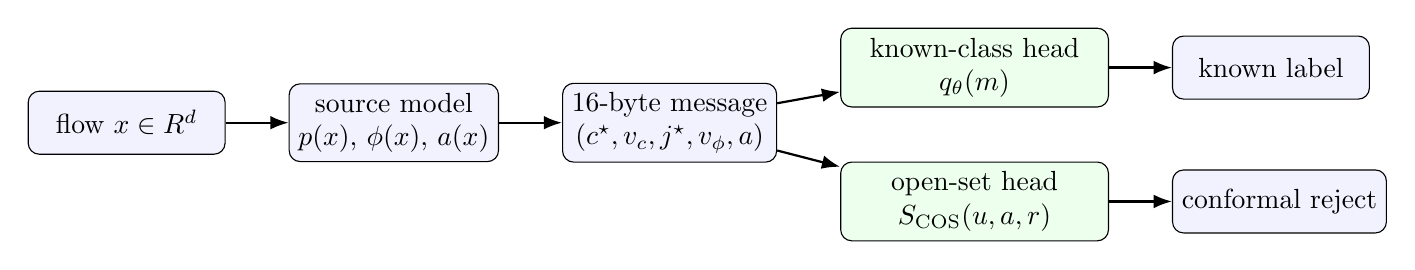
\begin{tikzpicture}[
node distance=7mm and 8mm,
box/.style={draw,rounded corners,align=center,minimum height=8mm,minimum width=25mm,fill=blue!5},
head/.style={draw,rounded corners,align=center,minimum height=10mm,minimum width=34mm,fill=green!7},
arr/.style={-Latex,thick}
]
\node[box] (flow) {flow $x\in\R^d$};
\node[box,right=of flow] (local) {source model\\$p(x)$, $\phi(x)$, $a(x)$};
\node[box,right=of local] (msg) {16-byte message\\$(c^\star,v_c,j^\star,v_\phi,a)$};
\node[head,right=of msg,yshift=7mm] (cls) {known-class head\\$q_\theta(m)$};
\node[head,right=of msg,yshift=-10mm] (open) {open-set head\\$S_{\rm COS}(u,a,r)$};
\node[box,right=of cls] (known) {known label};
\node[box,right=of open] (reject) {conformal reject};
\draw[arr] (flow)--(local);
\draw[arr] (local)--(msg);
\draw[arr] (msg)--(cls);
\draw[arr] (msg)--(open);
\draw[arr] (cls)--(known);
\draw[arr] (open)--(reject);
\end{tikzpicture}}
\caption{Revised \method{} architecture. $c^\star$ and $v_c$ denote the top class and probability; $j^\star$ and $v_\phi$ denote the top attribution-proxy feature and contribution; $a$ is local anomaly evidence. The classification and rejection heads are distinct.}
\label{fig:architecture}
\end{figure}


\section{Experimental Design}

\subsection{Datasets and leakage control}

The primary data are the encoded 5G-NIDD flows: 1,215,890 observations covering benign traffic and eight attack families \cite{siriwardhana2025descriptor}. The label counts are 477,737 Benign, 140,812 HTTPFlood, 1,155 ICMPFlood, 9,721 SYNFlood, 20,043 SYNScan, 73,124 SlowrateDoS, 20,052 TCPConnectScan, 457,340 UDPFlood, and 15,906 UDPScan.

Labels, attack-tool fields, scenario/order fields, and endpoint identifiers matching the leakage rules are excluded from predictive inputs. Numeric fields are median-imputed and standardized. Categorical fields are most-frequent imputed and one-hot encoded. The preprocessing model is fit only on the training partition. The source identifier \texttt{sVid} is retained solely for assigning ownership to eight monitor slots and is never a predictor.

The secondary CICIoT2023 stress test uses a transparent category-balanced-by-subattack sample generated from the complete CSV release \cite{neto2023ciciot}. It contains 10,000 Benign, 10,000 BruteForce, 119,967 DDoS, 39,982 DoS, 29,999 Mirai, 42,261 Recon, 19,999 Spoofing, and 24,829 Web observations. This experiment is not presented as a generalization success; it measures transfer limitations under a fixed encoding.

\subsection{Holdouts, splits, and seeds}

For every 5G-NIDD task, one attack family is excluded from all model fitting and used only as unknown test data. The remaining known observations are divided into 56\% training, 14\% validation, and 30\% known test data. Validation data calibrate normalization and the conformal rejection rule. The entire procedure is repeated for eight attack families and seeds $\{7,21,42,84,123\}$, giving 40 matched trials per method.

The CICIoT2023 experiment holds out each of seven attack categories once and uses seed 42. It is reported separately because its purpose is stress testing, not confirmatory inference.

\subsection{Models and baselines}

Each source classifier is a Random Forest with 30 trees, minimum leaf size 2, and balanced-subsample class weighting. Each source anomaly model is an Isolation Forest with 100 trees and automatic contamination. The known head is one-versus-rest logistic regression with balanced class weights and the liblinear solver.

The protocol-matched baselines are:
\begin{itemize}
    \item centralized full-feature Random Forest with entropy rejection;
    \item centralized full-feature Extra Trees with entropy rejection;
    \item centralized Random Forest with class-conditional extreme-value-theory (EVT) tail rejection, an OpenMax-style comparison;
    \item an all-source logit-average plus anomaly score;
    \item a five-round FedAvg linear classifier;
    \item \dhmethod{}, which uses the same 24-byte message but coordinator uncertainty only;
    \item message-content, precision, size, and score-component ablations.
\end{itemize}
Published deep and federated IDS methods are discussed in Section~2, but we do not report their published closed-set numbers as direct competitors because the data splits, unknown-family definitions, and communication accounting differ.

\subsection{Metrics and statistical analysis}

Known classification is measured by macro-F1. Unknown ranking is measured by AUROC. Operational recall is measured using the split-conformal $\alpha=0.05$ rule, and the resulting known-test FPR is reported. We also report TPR at a test-set FPR of 5\% as a ranking diagnostic, but it is not used as the operational threshold.

Comparisons use matched seed--holdout pairs. We report paired $t$-tests, Wilcoxon signed-rank tests \cite{wilcoxon1945}, Holm-adjusted p-values \cite{holm1979}, rank-biserial effects, and bootstrap 95\% confidence intervals \cite{efron1993bootstrap}. The family of 20 method--metric tests is corrected jointly.

\subsection{Computational accounting}

The experiments were executed on an Apple M4 Max workstation with 14 logical CPU cores and 36 GiB of memory, running macOS 26.6.2 (arm64), Python 3.12.9, NumPy 2.5.0, pandas 3.0.3, SciPy 1.18.1, scikit-learn 1.9.0, SHAP 0.52.0, joblib 1.6.0, and Matplotlib 3.11.1. All methods in the protocol-matched comparison were evaluated in the same software environment and on the same machine.

The measured latency is coordinator prediction time divided by the number of known and unknown test flows; it is not end-to-end device or network latency. Serialized model artifacts are measured with joblib. The aggregate X-MAG-COS artifact (eight source classifiers, eight anomaly models, and coordinator) is approximately 10.4 MiB; the centralized Random Forest is 3.57 MiB and Extra Trees is 24.16 MiB. Thus, the evidence message is communication-compact, but the aggregate model is not smaller than every centralized baseline.


\section{Protocol-Matched 5G-NIDD Results}

\subsection{Overall performance and family dependence}

Table~\ref{tab:familymain} reports the five-seed result for \compactmethod{}. Known-class macro-F1 is consistently high. Open-set performance, however, is family-dependent. HTTPFlood, ICMPFlood, SYNFlood, and SYNScan are well separated. UDPFlood is not: its mean AUROC is 0.4533 and its conformal recall is 0.0032. SlowrateDoS and TCPConnectScan are intermediate. Figure~\ref{fig:family} adds the seed-to-seed dispersion, and Section~\ref{sec:harddiagnostics} uses retained per-flow scores from the detection-equivalent 24-byte reference to explain the two most difficult families.

\begin{table}[H]
\caption{Five-seed 5G-NIDD performance of \compactmethod{}. Values are mean $\pm$ standard deviation across seeds. Recall and FPR use the split-conformal 5\% rule.}
\label{tab:familymain}
\centering
\small
\begin{tabular}{lrrrr}
\toprule
Held-out family & Known macro-F1 & Unknown AUROC & Unknown recall & Known FPR \\
\midrule
HTTPFlood & $0.9991\pm0.0001$ & $0.9894\pm0.0023$ & $0.9447\pm0.0123$ & $0.0504\pm0.0003$ \\
ICMPFlood & $0.9986\pm0.0001$ & $0.9966\pm0.0021$ & $1.0000\pm0.0000$ & $0.0494\pm0.0008$ \\
SlowrateDoS & $0.9991\pm0.0001$ & $0.8994\pm0.0185$ & $0.3035\pm0.1161$ & $0.0499\pm0.0006$ \\
SYNFlood & $0.9984\pm0.0003$ & $0.9924\pm0.0021$ & $1.0000\pm0.0000$ & $0.0496\pm0.0003$ \\
SYNScan & $0.9988\pm0.0003$ & $0.9958\pm0.0014$ & $1.0000\pm0.0000$ & $0.0499\pm0.0008$ \\
TCPConnectScan & $0.9988\pm0.0001$ & $0.9268\pm0.0495$ & $0.7119\pm0.2734$ & $0.0497\pm0.0002$ \\
UDPFlood & $0.9985\pm0.0001$ & $0.4533\pm0.0146$ & $0.0032\pm0.0044$ & $0.0496\pm0.0003$ \\
UDPScan & $0.9988\pm0.0001$ & $0.9643\pm0.0261$ & $0.8274\pm0.1614$ & $0.0492\pm0.0002$ \\
\midrule
All 40 trials & $0.9987\pm0.0003$ & $0.9022\pm0.1763$ & $0.7238\pm0.3714$ & $0.0497\pm0.0006$ \\
\bottomrule
\end{tabular}
\end{table}

\begin{figure}[H]
\centering
\includegraphics[width=0.86\textwidth]{figures/per_family_5g.pdf}
\caption{Five-seed open-set performance of \compactmethod{} by held-out 5G-NIDD family. Bars show means and error bars show one standard deviation. The figure exposes the family dependence hidden by the overall mean, particularly for SlowrateDoS, TCPConnectScan, UDPFlood, and UDPScan.}
\label{fig:family}
\end{figure}

\subsection{Controlled baseline comparison}

Every row of Table~\ref{tab:baselines} uses the same 40 splits and conformal 5\% rule. The centralized Random Forest is a strong full-feature reference. Its mean recall is higher than that of \compactmethod{}, whereas its mean AUROC is lower; neither open-set difference is significant after Holm correction. \compactmethod{} is therefore not claimed to dominate the centralized model. Its principal advantage is a 16-byte evidence payload instead of a 352-byte transformed vector, a 95.5\% reduction.

The all-source logit average performs poorly on known classes under the source-aware non-IID ownership. This result demonstrates that simple averaging is not a suitable distributed comparator in this protocol, rather than implying that all distributed IDS methods fail. FedAvg preserves moderate open-set ranking but loses known-class macro-F1.

\begin{table}[H]
\caption{Protocol-matched comparison over eight 5G-NIDD holdouts and five seeds ($n=40$). All recall and FPR values use the split-conformal 5\% rule. ``Bytes'' denotes inference-time evidence/feature payload; FedAvg exchanges model updates during training and is therefore not assigned a per-flow payload.}
\label{tab:baselines}
\centering
\scriptsize
\begin{tabular}{L{0.25\textwidth}rrrrrr}
\toprule
Method & Bytes & Known F1 & AUROC & Recall & Mean FPR & Coordinator $\mu$s/flow \\
\midrule
\compactmethod{} & 16 & 0.9987 & 0.9022 & 0.7238 & 0.0497 & 0.959 \\
\referencemethod{} & 24 & 0.9987 & 0.9022 & 0.7238 & 0.0497 & 0.929 \\
\dhmethod{} & 24 & 0.9987 & 0.9050 & 0.7042 & 0.0498 & 0.929 \\
All-source logit average & 36 & 0.0753 & 0.8505 & 0.5104 & 0.0499 & 0.355 \\
FedAvg linear & -- & 0.9013 & 0.9004 & 0.6600 & 0.0500 & 0.232 \\
Central Random Forest & 352 & 0.9988 & 0.8873 & 0.7986 & 0.0348 & 0.339 \\
Central Extra Trees & 352 & 0.9941 & 0.8868 & 0.6182 & 0.0489 & 0.466 \\
Central RF + EVT tail & 352 & 0.9988 & 0.7886 & 0.3979 & 0.0503 & 0.339 \\
\bottomrule
\end{tabular}
\end{table}

\subsection{Communication--performance frontier}

The 16-byte encoding retains the performance of the 24-byte reference. Across 40 matched trials, its mean differences relative to 24B are $-2.5\times10^{-7}$ macro-F1, $6.7\times10^{-6}$ AUROC, and $2.4\times10^{-5}$ recall. The corresponding paired $t$-test p-values are 0.323, 0.161, and 0.600; the Wilcoxon p-values are 0.317, 0.646, and 0.730. The quantized encoding is therefore the compact Pareto operating point in the evaluated family. The 20- and 24-byte rows carry the same predictive payload and differ only in framing; their quality is accordingly identical.

\begin{table}[H]
\caption{Five-seed communication ablation over 40 matched trials. The full-feature row transmits all transformed float32 features.}
\label{tab:pareto}
\centering
\begin{tabular}{lrrrr}
\toprule
Encoding & Bytes & Known F1 & Unknown AUROC & Unknown recall \\
\midrule
Class+anomaly & 12 & 0.9987 & 0.9007 & 0.7117 \\
\compactmethod{} & 16 & 0.9987 & 0.9022 & 0.7238 \\
Class+proxy & 18 & 0.9988 & 0.8980 & 0.7004 \\
X-MAG-COS-20B & 20 & 0.9987 & 0.9022 & 0.7238 \\
\referencemethod{} & 24 & 0.9987 & 0.9022 & 0.7238 \\
X-MAG-COS-30B & 30 & 0.9988 & 0.8991 & 0.6883 \\
Central full features & 352 & 0.9988 & 0.8873 & 0.7986 \\
\bottomrule
\end{tabular}
\end{table}

\begin{figure}[H]
\centering
\includegraphics[width=0.82\textwidth]{figures/pareto_auroc.pdf}
\caption{Communication--performance frontier over 40 matched trials. The horizontal axis uses a logarithmic scale to display the 12--36-byte evidence messages together with the 352-byte centralized feature vector. The 16-byte message is the smallest evaluated full-content encoding and is indistinguishable in quality from the 24-byte reference.}
\label{fig:pareto}
\end{figure}

\subsection{Hard-family diagnostic evidence}
\label{sec:harddiagnostics}

The communication frontier establishes that quantization is not responsible for the difficult-family behavior: the 16-byte and 24-byte full-content encodings have indistinguishable aggregate detection quality. The retained per-flow diagnostic arrays were generated for the 24-byte float32 reference and are therefore used only to examine the failure mechanism. Receiver operating characteristic (ROC) curves are threshold-free. For the score-distribution and missed-decision analyses, a validation 95th-percentile threshold was used; its mean known-traffic false-positive rates were 0.0496 for UDPFlood and 0.0500 for SlowrateDoS, closely matching the nominal 5\% operating point.

Figure~\ref{fig:hardroc} shows qualitatively different behavior for the two families. SlowrateDoS retains useful ranking information (mean AUROC $0.8994\pm0.0185$), although its thresholded recall is only $0.3035\pm0.1162$. UDPFlood is below random ranking on average (AUROC $0.4533\pm0.0146$) and is almost never rejected (recall $0.0032\pm0.0044$). Figure~\ref{fig:hardhist} explains this contrast: SlowrateDoS scores are shifted toward the upper part of the range but still overlap known traffic near the operating threshold, whereas UDPFlood scores overlap the low-score known-traffic region extensively.

\begin{figure}[H]
\centering
\subfloat[UDPFlood.]{\includegraphics[width=0.49\textwidth]{figures/roc_udpflood.pdf}}
\hfill
\subfloat[SlowrateDoS.]{\includegraphics[width=0.49\textwidth]{figures/roc_slowratedos.pdf}}
\caption{Five-seed open-set ROC diagnostics for the two difficult 5G-NIDD holdouts using the detection-equivalent 24-byte float32 reference. The solid curve is the seed mean, the band is one standard deviation, and the diagonal denotes random ranking. The vertical line marks a false-positive rate of 0.05 for visual reference.}
\label{fig:hardroc}
\end{figure}

\begin{figure}[H]
\centering
\subfloat[UDPFlood.]{\includegraphics[width=0.49\textwidth]{figures/score_histogram_udpflood.pdf}}
\hfill
\subfloat[SlowrateDoS.]{\includegraphics[width=0.49\textwidth]{figures/score_histogram_slowratedos.pdf}}
\caption{Composite-score distributions for known test traffic and the held-out families, pooled from five seed evaluations of the 24-byte reference. UDPFlood occupies the same low-score region as much of the known traffic, whereas SlowrateDoS is more strongly shifted but retains substantial overlap around the operating threshold.}
\label{fig:hardhist}
\end{figure}

The class assignments of missed held-out decisions further distinguish the mechanisms (Figure~\ref{fig:hardassign}). Across the five seed evaluations, all 2,279,445 accepted UDPFlood decisions were assigned to Benign. Among 254,662 accepted SlowrateDoS decisions, 253,875 (99.691\%) were assigned to HTTPFlood and 787 (0.309\%) to Benign. These are repeated seed-trial decisions over the same held-out records rather than counts of unique flows. The SlowrateDoS error therefore supports absorption into a semantically related application-layer flooding class. The UDPFlood error does not: it is a joint representation and rejection failure in which the held-out traffic appears benign to the compact known-class head and receives low composite scores.

\begin{figure}[H]
\centering
\includegraphics[width=0.78\textwidth]{figures/accepted_unknown_assignments.pdf}
\caption{Known-class assignments for held-out decisions that fell below the validation 95th-percentile rejection threshold, aggregated over five seeds. All missed UDPFlood decisions were assigned to Benign, whereas 99.691\% of missed SlowrateDoS decisions were assigned to HTTPFlood.}
\label{fig:hardassign}
\end{figure}


\section{Composite-Score Analysis}

\subsection{Component and head ablations}

Table~\ref{tab:scoreablation} does not support a claim that the composite score is universally superior. Coordinator uncertainty achieves a slightly larger mean AUROC, while the composite score provides a 0.0196 mean recall gain. The paired differences are not significant after Holm correction. The defensible conclusion is that the composite construction provides a recall-oriented balanced operating score whose individual signals have interpretable roles. Anomaly-only and residual-only scores are insufficient.

\begin{table}[H]
\caption{Open-set score ablation with the same 24-byte message, five seeds, and eight holdouts.}
\label{tab:scoreablation}
\centering
\begin{tabular}{lrrrr}
\toprule
Open-set score & Mean AUROC & Min AUROC & Mean recall & Min recall \\
\midrule
Composite $S_{\rm COS}$ & 0.9022 & 0.4401 & 0.7238 & 0.0000 \\
Coordinator uncertainty & 0.9050 & 0.3838 & 0.7042 & 0.0000 \\
Uncertainty+anomaly & 0.9014 & 0.4563 & 0.7056 & 0.0000 \\
Anomaly only & 0.8296 & 0.5524 & 0.0270 & 0.0000 \\
Message residual only & 0.7711 & 0.3099 & 0.0000 & 0.0000 \\
\bottomrule
\end{tabular}
\end{table}

\subsection{Hyperparameter sensitivity}

The reference weights were fixed after the exploratory development stage and before the five-seed confirmatory rerun. The full $5^3$ grid uses $\{0,0.25,0.5,0.75,1\}$ for each parameter. The selected point obtains mean AUROC 0.9022 and mean recall 0.7238. The largest mean AUROC is 0.9045 at $\lambda=0.75,\gamma=0$ (independent of $\beta$), with recall 0.7148. The largest mean recall is 0.7281 at $(\beta,\lambda,\gamma)=(0.25,0.50,0.75)$, with AUROC 0.8960. Thus, the selected score lies within 0.0023 AUROC of the best ranking point and within 0.0043 recall of the best recall point. No grid point solves UDPFlood: the minimum family recall remains zero.

\begin{table}[H]
\caption{Representative composite-score settings over 40 matched trials.}
\label{tab:sensitivity}
\centering
\begin{tabular}{lrrrrrr}
\toprule
Setting & $\beta$ & $\lambda$ & $\gamma$ & Mean AUROC & Mean recall & Max FPR \\
\midrule
Reference compromise & 0.25 & 0.50 & 0.25 & 0.9022 & 0.7238 & 0.0518 \\
Highest mean AUROC & 0.00 & 0.75 & 0.00 & 0.9045 & 0.7148 & 0.0514 \\
Highest mean recall & 0.25 & 0.50 & 0.75 & 0.8960 & 0.7281 & 0.0512 \\
Anomaly branch only & 0.00 & 0.00 & 0.00 & 0.8296 & 0.0667 & 0.0513 \\
\bottomrule
\end{tabular}
\end{table}

\begin{figure}[H]
\centering
\includegraphics[width=0.82\textwidth]{figures/sensitivity_auroc.pdf}
\caption{Sensitivity of mean AUROC to the composite-score weights. The selected setting belongs to a broad high-performing region rather than a sharp isolated optimum.}
\label{fig:sensitivity}
\end{figure}

\subsection{Paired statistical comparisons}

Table~\ref{tab:statistics} reports selected paired comparisons for the 24-byte float32 reference; Section~6.3 establishes its detection equivalence to 16Q. Relative to the all-source logit ensemble, X-MAG-COS improves AUROC and recall significantly after Holm correction. Relative to the centralized Random Forest, the open-set differences are not significant. Relative to \dhmethod{}, neither the small AUROC decrease nor the small recall increase is significant. These results limit the supported claim to a communication-efficient operating point rather than universal statistical superiority.

\begin{table}[H]
\caption{Selected paired tests over 40 seed--holdout pairs. Confidence intervals are bootstrap 95\% intervals for X-MAG-COS-24B minus the comparator; $p_{\rm W,H}$ is the Holm-adjusted Wilcoxon p-value.}
\label{tab:statistics}
\centering
\scriptsize
\begin{tabular}{L{0.25\textwidth}lrrr}
\toprule
Comparator & Metric & Mean difference [95\% CI] & $p_{\rm W,H}$ \\
\midrule
\dhmethod{} & AUROC & $-0.0028$ [$-0.0082$, $0.0034$] & 0.162 \\
\dhmethod{} & Recall & $0.0196$ [$-0.0026$, $0.0409$] & 0.224 \\
All-source logit average & AUROC & $0.0517$ [$0.0305$, $0.0736$] & $<0.001$ \\
All-source logit average & Recall & $0.2134$ [$0.0834$, $0.3421$] & 0.015 \\
Central Random Forest & AUROC & $0.0149$ [$-0.0413$, $0.0757$] & 1.000 \\
Central Random Forest & Recall & $-0.0748$ [$-0.1499$, $-0.0058$] & 1.000 \\
FedAvg linear & Known F1 & $0.0974$ [$0.0801$, $0.1142$] & $<0.001$ \\
Central Extra Trees & Known F1 & $0.0046$ [$0.0025$, $0.0071$] & $<0.001$ \\
\bottomrule
\end{tabular}
\end{table}

\section{Attribution-Proxy Fidelity and Cost}

The TreeSHAP comparison is deliberately limited to the two difficult held-out families and seed 42. Table~\ref{tab:shap} shows high absolute-rank Spearman correlation but only moderate exact top-1 agreement. The proxy therefore preserves broad feature ordering better than exact per-flow feature identity. This evidence supports the term ``attribution-aware'' but not an equivalence claim with SHAP or LIME.

\begin{table}[H]
\caption{Attribution-proxy agreement with TreeSHAP. Top-3 overlap is the mean Jaccard similarity.}
\label{tab:shap}
\centering
\begin{tabular}{lrrrrr}
\toprule
Holdout & Samples & Top-1 agreement & Top-3 overlap & Rank $\rho$ & Speedup \\
\midrule
UDPFlood & 1,896 & 0.271 & 0.650 & 0.937 & $156.7\times$ \\
SlowrateDoS & 1,851 & 0.409 & 0.416 & 0.908 & $73.1\times$ \\
\bottomrule
\end{tabular}
\end{table}

The proxy requires approximately 0.028 s for each sampled hard-holdout set, whereas TreeSHAP requires 2.03--4.33 s. This cost difference motivates the proxy for per-flow evidence generation. The modest top-1 agreement remains a limitation: the transmitted field is a ranking surrogate, not a complete local explanation.

\section{Channel Artifacts and Targeted Evidence Manipulation}

\subsection{Exploratory peer-context simulation}

To move beyond independent deterministic partitions, we evaluated an optional coordinator input that concatenates each owner message with the pooled latest delivered messages from the other source monitors. Packet loss and bounded event-order jitter emulate channel artifacts. Table~\ref{tab:network} shows that naive peer pooling is not robust: performance changes non-monotonically and often collapses under small loss/jitter. This negative result prevents us from presenting peer-context fusion as a validated contribution.

\begin{table}[H]
\caption{Exploratory pooled-peer-context simulation at seed 42. Values use the conformal 5\% rule. The non-monotonic results indicate unstable score calibration under naive asynchronous pooling.}
\label{tab:network}
\centering
\small
\begin{tabular}{llrrrr}
\toprule
Holdout & Channel & Delivery & Known F1 & AUROC & Unknown recall \\
\midrule
\multirow{4}{*}{UDPFlood}
& Ideal & 1.000 & 0.9986 & 0.6763 & 0.0000 \\
& Edge (1\%, 3 steps) & 0.990 & 0.9838 & 0.3005 & 0.0102 \\
& Congested (5\%, 20 steps) & 0.950 & 0.9436 & 0.1346 & 0.0500 \\
& Severe (10\%, 50 steps) & 0.900 & 0.9516 & 0.8041 & 0.0000 \\
\midrule
\multirow{4}{*}{SlowrateDoS}
& Ideal & 1.000 & 0.9990 & 0.9873 & 1.0000 \\
& Edge (1\%, 3 steps) & 0.990 & 0.9270 & 0.2198 & 0.0136 \\
& Congested (5\%, 20 steps) & 0.951 & 0.9312 & 0.3165 & 0.0503 \\
& Severe (10\%, 50 steps) & 0.901 & 0.9020 & 0.4980 & 0.0000 \\
\bottomrule
\end{tabular}
\end{table}

\subsection{Active source compromise}

The targeted experiment compromises one active source monitor in each hard-holdout task. Because the ownership metadata occupies fewer active slots than the nominal eight, requested fractions of 10--30\% all selected the same one source; the study therefore supports a single-source-compromise conclusion, not a dose-response claim.

Class-evidence suppression, benign-message replay, and combined manipulation collapse known macro-F1 to 0.0966 for UDPFlood and 0.0737 for SlowrateDoS. Attribution replacement preserves known F1 but substantially changes rejection. Anomaly suppression reduces unknown recall to zero for UDPFlood and 0.0154 for SlowrateDoS. The method is consequently not robust to an authenticated source being malicious. Deployment requires message authentication, source attestation, reliability weighting, or redundant observation.

\begin{table}[H]
\caption{Targeted single-source compromise at seed 42. FPR is reported because some attacks obtain apparent recall by exceeding the 5\% known-traffic budget.}
\label{tab:active}
\centering
\scriptsize
\begin{tabular}{llrrrr}
\toprule
Holdout & Manipulation & Known F1 & AUROC & Recall & FPR \\
\midrule
\multirow{5}{*}{UDPFlood}
& Class suppression & 0.0966 & 0.6064 & 0.0000 & 0.0000 \\
& Attribution replacement & 0.9986 & 0.4822 & 0.0000 & 0.0462 \\
& Anomaly suppression & 0.9987 & 0.4664 & 0.0000 & 0.1490 \\
& Benign-message replay & 0.0966 & 0.6258 & 0.0000 & 0.0000 \\
& Combined & 0.0966 & 0.6296 & 0.0000 & 0.0000 \\
\midrule
\multirow{5}{*}{SlowrateDoS}
& Class suppression & 0.0737 & 0.9142 & 0.0033 & 0.0226 \\
& Attribution replacement & 0.9990 & 0.9238 & 0.5031 & 0.0820 \\
& Anomaly suppression & 0.9990 & 0.8855 & 0.0154 & 0.0208 \\
& Benign-message replay & 0.0737 & 0.9725 & 0.4819 & 0.0109 \\
& Combined & 0.0737 & 0.9160 & 0.0000 & 0.0075 \\
\bottomrule
\end{tabular}
\end{table}


\section{CICIoT2023 Transfer Stress Test}

The fixed 5G-NIDD design is transferred without category-specific retuning to seven CICIoT2023 attack-category holdouts. Table~\ref{tab:ciciot} shows that the stress test is difficult for all methods. The all-source logit ensemble obtains the largest mean AUROC and recall, although its known-class F1 remains below the centralized Random Forest. X-MAG-COS-16Q does not improve monotonically with additional bytes: the 24-byte row is numerically identical, while 30 bytes is worse. Thus, increasing the evidence payload by 4--14 bytes does not resolve the observed domain shift.

\begin{table}[H]
\caption{CICIoT2023 category-holdout stress test (seven categories, seed 42). Recall and FPR use the conformal 5\% rule. Full transformed features require 152 bytes.}
\label{tab:ciciot}
\centering
\scriptsize
\begin{tabular}{lrrrrr}
\toprule
Method & Bytes & Known F1 & AUROC & Recall & Mean FPR \\
\midrule
Class+anomaly & 12 & 0.7225 & 0.7032 & 0.2034 & 0.0498 \\
X-MAG-COS-16Q & 16 & 0.7224 & 0.7015 & 0.2061 & 0.0500 \\
Class+proxy & 18 & 0.7223 & 0.6236 & 0.1563 & 0.0499 \\
X-MAG-COS-24B & 24 & 0.7224 & 0.7015 & 0.2061 & 0.0500 \\
X-MAG-COS-30B & 30 & 0.7166 & 0.6777 & 0.1613 & 0.0506 \\
All-source logit average & 32 & 0.7409 & 0.7640 & 0.2406 & 0.0506 \\
Central Random Forest & 152 & 0.7447 & 0.7313 & 0.2135 & 0.0504 \\
FedAvg linear & -- & 0.5936 & 0.5918 & 0.0941 & 0.0502 \\
\bottomrule
\end{tabular}
\end{table}

\begin{figure}[H]
\centering
\includegraphics[width=0.84\textwidth]{figures/ciciot_per_category.pdf}
\caption{CICIoT2023 category-level performance of X-MAG-COS-16Q. DDoS, DoS, and Mirai remain poorly rejected; the experiment is a boundary test rather than evidence of broad cross-dataset generalization.}
\label{fig:ciciot}
\end{figure}

\section{Discussion}

\subsection{What the confirmatory evaluation establishes}

The revised evidence supports three conclusions. First, compact evidence can preserve known-class classification. The 16-byte message differs negligibly from the 24-byte float32 reference and from the centralized Random Forest in macro-F1. Second, the open-set problem remains attack-family dependent. High mean values do not compensate for the UDPFlood failure, which persists across five seeds and the full hyperparameter grid. Third, the composite head is not globally dominant over uncertainty alone. It provides a small recall-oriented tradeoff, whereas the broader contribution is the calibrated two-head architecture and explicit communication frontier.

\subsection{Why the two difficult families fail differently}

The per-flow diagnostics replace the earlier generic semantic-overlap hypothesis with measured evidence. For SlowrateDoS, the classifier assigns 99.691\% of missed decisions to HTTPFlood, and the score distribution is shifted upward despite overlap around the threshold. This is consistent with class absorption between two application-layer flooding behaviors. UDPFlood exhibits a different failure: all missed decisions are assigned to Benign, its mean AUROC is below 0.5, and its scores concentrate in the low-score region occupied by known traffic. Increasing message size or changing the composite weights does not repair this behavior. The likely remedy is therefore not a larger encoding of the same instantaneous statistics, but additional discriminative structure such as protocol-preserving temporal features, sequence models, class-conditional density estimates, or source-aware calibration. The distinction also explains why a single statement about ``semantically similar flooding attacks'' is insufficient for both families.

\subsection{Practical feasibility}

The 16-byte payload is implementable as an application message over current constrained-network transports. The actual end-to-end wire size will be larger after transport and security headers, and batching several flow messages may be more efficient than one packet per flow. The one- and two-byte identifiers are sufficient for the measured dimensions. Binary16 quantization produces no measurable detection loss in the present data. However, the aggregate local-model artifact is approximately 10.4 MiB, so the phrase ``lightweight endpoint model'' would be misleading without device-level profiling. The supported claim is \emph{communication-compact evidence messaging}.

\subsection{Relation to distributed IDS}

The source-aware design is closer to multi-source edge monitoring than to a general multi-agent coordination algorithm. Each flow has one owner, and the principal coordinator consumes that owner's message. The exploratory peer-context experiment shows that simply concatenating stale or missing peer messages is unstable. A genuine multi-agent extension should model observation overlap, asynchronous state, trust, and Byzantine-resilient aggregation explicitly.

\section{Limitations}

The primary limitation is unknown-family heterogeneity: UDPFlood is essentially undetected at the conformal operating point, and the diagnostic analysis shows that missed UDPFlood decisions are classified as Benign rather than merely confused with another flood class. Second, the attribution field is a proxy. Its rank correlation with TreeSHAP is high, but exact top-feature agreement is modest. Third, the main source-partitioned architecture does not provide robust cross-agent fusion, and the exploratory peer-context extension is brittle. Fourth, a single compromised active source can collapse class prediction or suppress unknown rejection. Fifth, CICIoT2023 confirms that adding bytes alone does not produce cross-domain transfer. Sixth, the total model artifact is larger than the centralized Random Forest, and the reported microsecond latency covers the coordinator only.


\section{Conclusions}

We presented \method{}, a calibrated, communication-constrained IDS that separates known-class classification from unknown-family rejection. The revised mathematical treatment defines a constrained multi-objective design, proves structural properties of the composite score, and provides finite-sample split-conformal false-positive control under exchangeability. In a source-aware, five-seed 5G-NIDD evaluation, the 16-byte half-precision encoding preserves known-class macro-F1 and is statistically indistinguishable in detection quality from the 24-byte reference while reducing the evidence payload by 95.5\% relative to the transformed full-feature vector. The same experiment also changes the paper's conclusion: X-MAG-COS does not dominate all full-feature or uncertainty-only baselines, and UDPFlood remains a decisive failure case. Attribution fidelity, channel artifacts, active source compromise, and CICIoT2023 transfer further delimit the claim. The supported contribution is therefore a compact and calibrated evidence-messaging design with transparent operating tradeoffs, not a universally superior or deployment-ready intrusion detector.

\authorcontributions{Conceptualization, methodology, software, validation, formal analysis, investigation, data curation, writing---original draft preparation, writing---review and editing, and visualization, all authors. All authors have read and agreed to the published version of the manuscript.}

% AUTHOR ACTION: insert the verified award number if the sponsor requires it.
\funding{This research was supported by the Cybersecurity Research and Innovation Pioneers Initiative, provided by the National Cybersecurity Authority (NCA) in the Kingdom of Saudi Arabia.}

\institutionalreview{Not applicable.}
\informedconsent{Not applicable.}

\dataavailability{Publicly available datasets were analyzed in this study. The 5G-NIDD dataset is available through IEEE DataPort at \url{https://doi.org/10.21227/xtep-hv36} and Fairdata at \url{https://doi.org/10.23729/e80ac9df-d9fb-47e7-8d0d-01384a415361}. CICIoT2023 is available from the Canadian Institute for Cybersecurity, University of New Brunswick. No new primary network-traffic data were collected. The source code, leakage-control rules, experiment configurations, and derived aggregate tables are available at \url{https://github.com/alqithami/xmag}. The original third-party datasets are not redistributed and must be obtained from their respective official sources under the applicable terms.}

\acknowledgments{Not applicable.}

\conflictsofinterest{The authors declare no conflicts of interest. The funder had no role in the design of the study; in the collection, analysis, or interpretation of the data; in the writing of the manuscript; or in the decision to publish the results.}

\abbreviations{Abbreviations}{
The following abbreviations are used in this manuscript:\\
\noindent
\begin{tabular}{@{}ll}
5G & fifth-generation mobile communication\\
AUROC & area under the receiver operating characteristic curve\\
CoAP & Constrained Application Protocol\\
EVT & extreme value theory\\
FL & federated learning\\
FPR & false-positive rate\\
IDS & intrusion detection system\\
IoT & Internet of Things\\
LIME & local interpretable model-agnostic explanations\\
MQTT & Message Queuing Telemetry Transport\\
OOD & out-of-distribution\\
SHAP & Shapley additive explanations\\
TPR & true-positive rate\\
XAI & explainable artificial intelligence
\end{tabular}
}

\appendixtitles{yes}
\appendixstart
\appendix

\section{Complete Statistical Test Results}

The complete paired test table, including paired $t$-tests, Wilcoxon tests, Holm corrections, rank-biserial effects, and bootstrap confidence intervals for all evaluated metrics, is supplied as supplementary data. The main text reports only comparisons necessary to interpret the claims.

\section{Reproducibility Parameters}

\begin{table}[H]
\caption{Confirmatory 5G-NIDD protocol.}
\centering
\begin{tabular}{ll}
\toprule
Element & Setting \\
\midrule
Holdouts & eight attack families, one held out at a time \\
Seeds & 7, 21, 42, 84, 123 \\
Known split & 56\% train, 14\% validation, 30\% test \\
Unknown split & entire held-out family used only for test \\
Monitor ownership & stable hash of leakage-excluded \texttt{sVid} into eight slots \\
Local classifier & Random Forest, 30 trees, min leaf 2, balanced subsample \\
Anomaly model & Isolation Forest, 100 trees, automatic contamination \\
Coordinator & balanced one-versus-rest logistic regression, liblinear \\
Threshold & split-conformal, $\alpha=0.05$ \\
Main message & 16-byte binary16 class/proxy/anomaly encoding \\
\bottomrule
\end{tabular}
\end{table}

\section{CICIoT2023 Category Detail}

\begin{table}[H]
\caption{Category-level X-MAG-COS-16Q results on the CICIoT2023 stress test (seed 42).}
\centering
\begin{tabular}{lrr}
\toprule
Held-out category & Unknown AUROC & Unknown recall \\
\midrule
BruteForce & 0.7978 & 0.2957 \\
DDoS & 0.6331 & 0.0639 \\
DoS & 0.3411 & 0.0004 \\
Mirai & 0.6371 & 0.0054 \\
Recon & 0.8705 & 0.4653 \\
Spoofing & 0.8311 & 0.2802 \\
Web & 0.7997 & 0.3317 \\
\bottomrule
\end{tabular}
\end{table}

\section{Software and Result Availability}

The repository contains the analysis scripts used to produce the five-seed protocol-matched results, sensitivity analysis, statistical tests, attribution-fidelity measurements, message serializers, and exploratory stress tests. Aggregate outputs are provided as supplementary data. Raw third-party datasets are excluded.

\reftitle{References}


\bibliography{reference_part1,reference_part2}
\end{document}
